\chapter{HASIL PERCOBAAN DAN ANALISIS}
\label{bab:hasil-percobaan-dan-analisis}

Bab ini menyajikan hasil pelaksanaan eksperimen yang dirancang pada Bab~\ref{bab:perancangan-sistem}. Pembahasan mencakup kinerja sumber, kebutuhan komputasi, perbandingan konfigurasi label, dan pengujian pada citra jalan Indonesia. Skenario, hasil numerik, dan analisis dipisahkan agar hubungan antara prosedur pengujian dan interpretasinya dapat ditelusuri. Seluruh nilai berasal dari eksperimen yang telah dilaksanakan.

\section{Skenario Percobaan}
\subsection{Perbandingan deteksi dan efisiensi pada domain sumber}
Skenario pertama membandingkan YOLOv8n, YOLOv12n, YOLO26n, rekonstruksi YOLOv8-PD, dan rekonstruksi YOLO-RD. Kelima model dilatih pada 6.777 citra sumber dengan enam kategori. Sebanyak 1.898 citra validasi digunakan untuk pemilihan bobot dan penghentian dini. Evaluasi akhir menggunakan 995 citra uji dengan 2.425 anotasi, sesuai Tabel~\ref{tab:pembagian}.

Riwayat pelatihan digunakan untuk membaca perkembangan metrik validasi, epoch terbaik, dan durasi pelatihan. Hasil uji dilaporkan melalui presisi, \textit{recall}, mAP@0,5, mAP@0,5:0,95, serta F1 makro. AP per kelas melengkapi nilai agregat agar kelemahan kategori tertentu tidak tertutup oleh rata-rata. Parameter, GFLOPs, dan estimasi FPS digunakan untuk menilai kebutuhan komputasi.

Analisis tambahan memisahkan data uji menurut negara sumber. Subset Tiongkok, Jepang, dan India masing-masing memuat 180, 705, dan 110 citra. Perbandingan menggunakan empat kategori kerusakan yang sama. Ketiga negara telah tercakup dalam pelatihan, sehingga pengujian ini merupakan evaluasi subkelompok sumber dan bukan pengujian pada negara yang belum pernah dilihat model.

\subsection{Perbandingan pelatihan empat dan enam kelas}
Skenario kedua membandingkan model utama dengan model yang dilatih setelah anotasi penutup saluran dan jalan bertambal dihapus. Citra serta pembagian datanya dipertahankan. Evaluasi kedua konfigurasi dibatasi pada D00, D10, D20, dan D40, dengan 2.035 anotasi uji. Dengan demikian, perubahan mAP tidak berasal dari perubahan jumlah kelas yang dirata-ratakan.

Pemeriksaan tambahan menghitung kotak prediksi lubang yang bertumpang tindih dengan anotasi pengecoh. Ambang kepercayaan ditetapkan 0,25 dan ambang IoU 0,5, mengikuti protokol Bab~\ref{bab:perancangan-sistem}. Terdapat 390 anotasi pengecoh pada data uji, terdiri atas 321 penutup saluran dan 69 jalan bertambal. Keluaran pemeriksaan berupa jumlah kotak prediksi, bukan persentase objek yang salah diklasifikasikan.

\subsection{Pengujian zero-shot pada citra jalan Indonesia}
Skenario ketiga menerapkan bobot terbaik pelatihan enam kelas pada 307 citra target tanpa \textit{fine-tuning}. Seluruh citra dipertahankan, termasuk 39 citra tanpa anotasi objek. Perbandingan utama sumber dan target menggunakan empat kelas kerusakan. Pada target, keempat kelas tersebut memiliki 481 anotasi.

Penurunan kinerja dihitung dalam poin persentase dan persentase relatif menggunakan Persamaan~\eqref{eq:gap-absolut} serta~\eqref{eq:gap-relatif}. Evaluasi tambahan menyertakan 21 anotasi jalan bertambal, sehingga mencakup lima kelas bersama. Hasil tambahan ini dipisahkan dari perbandingan utama. Penutup saluran tidak dinilai pada target karena tidak memiliki anotasi.

Contoh prediksi target ditampilkan dengan ambang kepercayaan 0,25 untuk membantu pembacaan visual. Nilai ini berbeda dari ambang minimum 0,001 pada penghitungan AP. Karena itu, kotak yang terlihat pada contoh bukan seluruh prediksi yang membentuk kurva presisi--\textit{recall} dalam evaluasi AP.

\section{Hasil Percobaan}
\subsection{Perkembangan dan durasi pelatihan}
\label{subsec:b4-pelatihan}
Ringkasan pelatihan utama disajikan pada Tabel~\ref{tab:b4-pelatihan}. Epoch terbaik mengikuti puncak mAP@0,5:0,95 validasi dalam riwayat pelatihan dan sesuai dengan catatan pemilihan bobot pada eksperimen. Durasi diperoleh dari waktu kumulatif pada akhir riwayat masing-masing model.
% Generated by scripts/paper/thesis_bab4_assets.py; see build/bab4-qa/evidence.json.
\begin{table}[H]
\centering
\caption{Ringkasan pelaksanaan pelatihan utama enam kelas.}
\label{tab:b4-pelatihan}
\begingroup\fontsize{10}{13}\selectfont
\setlength{\tabcolsep}{3pt}
\begin{tabularx}{\linewidth}{|X|r|r|r|}\hline
\rowcolor{black}\HeaderTabel{Model}&\HeaderTabel{Epoch terbaik}&\HeaderTabel{Epoch akhir}&\HeaderTabel{Waktu (jam)}\\\hline
YOLOv8n & 108 & 148 & 4,36\\\hline
YOLOv12n & 110 & 150 & 4,66\\\hline
YOLO26n & 131 & 171 & 5,28\\\hline
YOLOv8-PD & 150 & 190 & 6,32\\\hline
YOLO-RD & 238 & 278 & 11,70\\\hline
\end{tabularx}\endgroup
\end{table}

Tabel~\ref{tab:b4-pelatihan} menunjukkan bahwa seluruh pelatihan berhenti sebelum batas 300 epoch. Selisih epoch terbaik dan epoch akhir adalah 40 pada setiap model, sesuai konfigurasi penghentian dini. YOLOv8n menyelesaikan 148 epoch dalam 4,36 jam, sedangkan YOLO-RD menyelesaikan 278 epoch dalam 11,70 jam. Durasi tersebut mencakup proses pelatihan beserta validasi yang tercatat selama proses berjalan.

Perkembangan metrik validasi disajikan pada Gambar~\ref{fig:b4-kurva}. Kedua panel menggunakan riwayat epoch asli tanpa penghalusan atau perpanjangan kurva setelah pelatihan berakhir.
\begin{figure}[H]
\centering
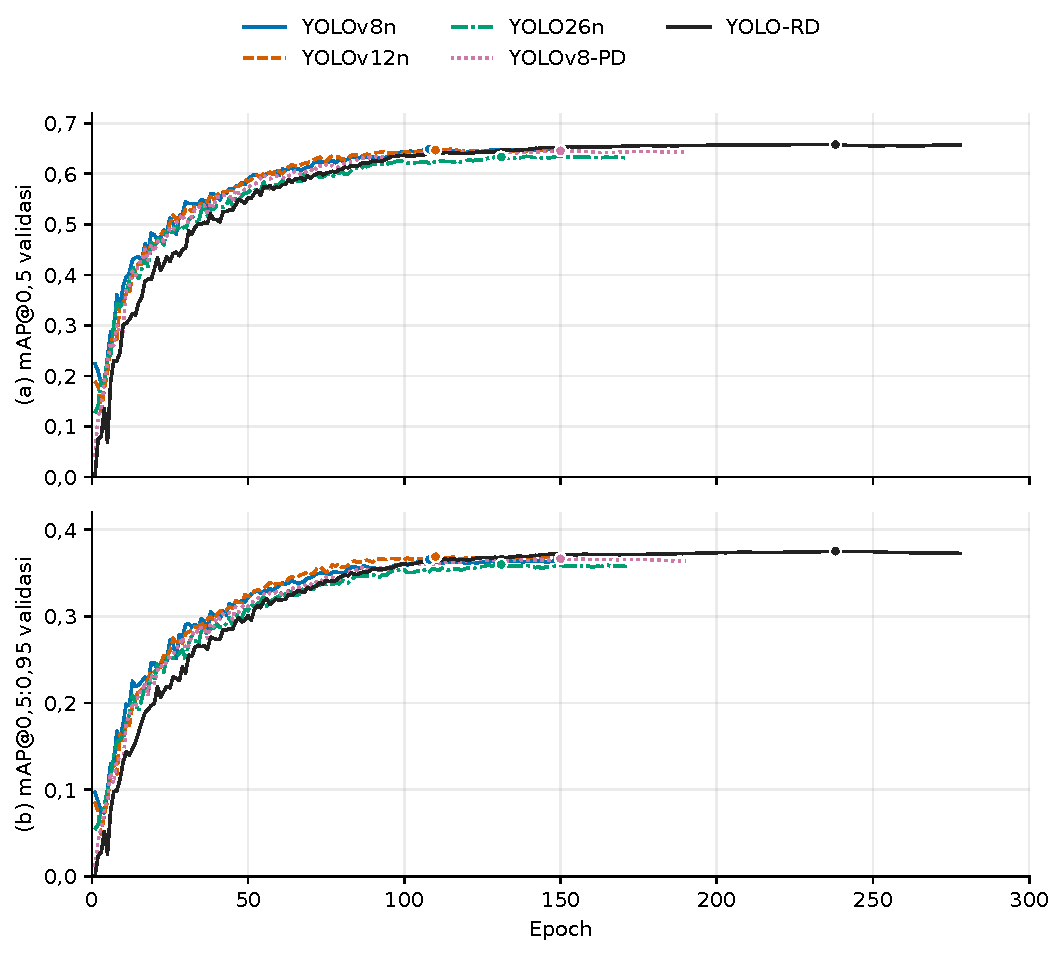
\includegraphics[width=\linewidth]{bab4-kurva-validasi.pdf}
\caption{Perkembangan mAP validasi pada pelatihan enam kelas. Titik menandai epoch terbaik berdasarkan mAP@0,5:0,95 validasi.}
\label{fig:b4-kurva}
\end{figure}
Gambar~\ref{fig:b4-kurva} memperlihatkan peningkatan metrik yang lebih besar pada bagian awal pelatihan, kemudian perubahan yang semakin kecil menjelang akhir. Model rekonstruksi memulai pelatihan dengan nilai validasi yang lebih rendah dan mencapai epoch terbaik lebih lambat. Kurva ini digunakan untuk menjelaskan proses pemilihan bobot, bukan menggantikan hasil pengujian akhir atau membuktikan terjadinya \textit{overfitting}.

\subsection{Kinerja deteksi pada data uji sumber}
Hasil agregat enam kelas disajikan pada Tabel~\ref{tab:b4-sumber}. Semua metrik dinyatakan pada skala nol sampai satu. Presisi dan \textit{recall} merupakan rata-rata kelas dari evaluator. F1 makro dirata-ratakan setelah F1 setiap kelas dihitung, bukan dari rata-rata presisi dan \textit{recall}.
% Generated by scripts/paper/thesis_bab4_assets.py; see build/bab4-qa/evidence.json.
\begin{table}[H]
\centering
\caption{Hasil pengujian sumber pada enam kelas.}
\label{tab:b4-sumber}
\begingroup\fontsize{10}{13}\selectfont
\setlength{\tabcolsep}{3pt}
\begin{tabularx}{\linewidth}{|X|r|r|r|r|r|}\hline
\rowcolor{black}\HeaderTabel{Model}&\HeaderTabel{Presisi}&\HeaderTabel{Recall}&\HeaderTabel{mAP@0,5}&\HeaderTabel{mAP@0,5:0,95}&\HeaderTabel{F1 makro}\\\hline
YOLOv8n & 0,643 & 0,599 & 0,648 & 0,364 & 0,617\\\hline
YOLOv12n & 0,638 & 0,608 & 0,654 & 0,371 & 0,619\\\hline
YOLO26n & 0,642 & 0,580 & 0,625 & 0,358 & 0,606\\\hline
YOLOv8-PD & 0,675 & 0,591 & 0,646 & 0,362 & 0,627\\\hline
YOLO-RD & 0,655 & 0,618 & 0,661 & 0,371 & 0,633\\\hline
\end{tabularx}\endgroup
\end{table}

Tabel~\ref{tab:b4-sumber} menunjukkan bahwa YOLO-RD memperoleh mAP@0,5 tertinggi sebesar 0,661 serta F1 makro tertinggi sebesar 0,633. YOLOv12n memperoleh mAP@0,5 sebesar 0,654. Pada mAP@0,5:0,95, kedua model bernilai 0,371 setelah pembulatan tiga desimal. YOLOv8-PD memiliki presisi tertinggi sebesar 0,675, sedangkan \textit{recall} tertinggi diperoleh YOLO-RD sebesar 0,618.

Rincian AP disajikan pada Tabel~\ref{tab:b4-kelas-sumber}. Identitas D00, D10, D20, D40, D70, dan D80 masing-masing merujuk pada retak memanjang, retak melintang, retak buaya, lubang, penutup saluran, dan jalan bertambal.
% Generated by scripts/paper/thesis_bab4_assets.py; see build/bab4-qa/evidence.json.
\begin{table}[H]
\centering
\caption{AP@0,5 per kelas pada data uji sumber.}
\label{tab:b4-kelas-sumber}
\begingroup\fontsize{10}{13}\selectfont
\setlength{\tabcolsep}{3pt}
\begin{tabularx}{\linewidth}{|X|r|r|r|r|r|r|}\hline
\rowcolor{black}\HeaderTabel{Model}&\HeaderTabel{D00}&\HeaderTabel{D10}&\HeaderTabel{D20}&\HeaderTabel{D40}&\HeaderTabel{D70}&\HeaderTabel{D80}\\\hline
YOLOv8n & 0,664 & 0,599 & 0,700 & 0,526 & 0,825 & 0,571\\\hline
YOLOv12n & 0,680 & 0,582 & 0,708 & 0,535 & 0,833 & 0,587\\\hline
YOLO26n & 0,639 & 0,567 & 0,675 & 0,538 & 0,820 & 0,512\\\hline
YOLOv8-PD & 0,678 & 0,572 & 0,702 & 0,541 & 0,819 & 0,562\\\hline
YOLO-RD & 0,696 & 0,608 & 0,701 & 0,527 & 0,845 & 0,587\\\hline
\end{tabularx}\endgroup
\end{table}

Tabel~\ref{tab:b4-kelas-sumber} menunjukkan bahwa penutup saluran memiliki AP@0,5 tertinggi pada setiap model, dengan rentang 0,819--0,845. Pada kelas lubang, nilainya berkisar 0,526--0,541. YOLOv8-PD mencapai AP lubang tertinggi, meskipun bukan pemilik mAP enam kelas tertinggi. Hasil ini memperlihatkan bahwa urutan model berdasarkan rata-rata tidak selalu sama dengan urutan pada satu kategori.

\subsection{Kompleksitas dan kecepatan pemrosesan}
Tabel~\ref{tab:b4-efisiensi} menyajikan kompleksitas model \textit{fused} pada masukan 640 piksel serta estimasi FPS sumber. Kompleksitas mengikuti penghitungan ulang \textit{checkpoint} akhir dengan Ultralytics 8.4.177. FPS mengikuti hasil validator pada RTX 4070 SUPER dan lingkungan pada Tabel~\ref{tab:lingkungan}.
% Generated by scripts/paper/thesis_bab4_assets.py; see build/bab4-qa/evidence.json.
\begin{table}[H]
\centering
\caption{Kompleksitas dan estimasi kecepatan model enam kelas.}
\label{tab:b4-efisiensi}
\begingroup\fontsize{10}{13}\selectfont
\setlength{\tabcolsep}{3pt}
\begin{tabularx}{\linewidth}{|X|r|r|r|}\hline
\rowcolor{black}\HeaderTabel{Model}&\HeaderTabel{Parameter (juta)}&\HeaderTabel{GFLOPs}&\HeaderTabel{FPS estimasi}\\\hline
YOLOv8n & 3,01 & 8,1 & 219,7\\\hline
YOLOv12n & 2,56 & 7,3 & 319,3\\\hline
YOLO26n & 2,38 & 5,3 & 293,3\\\hline
YOLOv8-PD & 2,47 & 7,7 & 368,4\\\hline
YOLO-RD & 7,09 & 12,8 & 189,4\\\hline
\end{tabularx}\endgroup
\end{table}

Tabel~\ref{tab:b4-efisiensi} memperlihatkan bahwa YOLO26n memiliki parameter dan GFLOPs paling rendah, masing-masing 2,38 juta dan 5,3. Estimasi FPS tertinggi diperoleh YOLOv8-PD sebesar 368,4, diikuti YOLOv12n sebesar 319,3. YOLO-RD memiliki parameter serta GFLOPs tertinggi dan estimasi FPS terendah pada pengukuran ini.

FPS dihitung dari waktu prapemrosesan, inferensi, dan pascapemrosesan sebelum pembulatan. Karena itu, perhitungan ulang dari waktu milidetik yang telah dibulatkan pada log dapat menghasilkan sedikit perbedaan. Angka kecepatan eksperimen tambahan empat kelas tidak digabungkan dalam tabel ini karena sebagian evaluasinya menggunakan GPU dan versi perangkat lunak berbeda.

\subsection{Kinerja menurut negara sumber}
Perbandingan negara disajikan pada Tabel~\ref{tab:b4-negara}. Rata-rata dibatasi pada empat kelas kerusakan untuk menghindari pengaruh perbedaan keberadaan kelas pengecoh. India tidak memiliki anotasi jalan bertambal dan hanya memiliki satu anotasi penutup saluran pada data uji.
% Generated by scripts/paper/thesis_bab4_assets.py; see build/bab4-qa/evidence.json.
\begin{table}[H]
\centering
\caption{mAP@0,5 empat kelas kerusakan menurut negara sumber.}
\label{tab:b4-negara}
\begingroup\fontsize{10}{13}\selectfont
\setlength{\tabcolsep}{3pt}
\begin{tabularx}{\linewidth}{|X|r|r|r|}\hline
\rowcolor{black}\HeaderTabel{Model}&\HeaderTabel{Tiongkok}&\HeaderTabel{Jepang}&\HeaderTabel{India}\\\hline
YOLOv8n & 0,931 & 0,578 & 0,284\\\hline
YOLOv12n & 0,933 & 0,579 & 0,293\\\hline
YOLO26n & 0,933 & 0,543 & 0,305\\\hline
YOLOv8-PD & 0,953 & 0,567 & 0,299\\\hline
YOLO-RD & 0,945 & 0,587 & 0,304\\\hline
\end{tabularx}\endgroup
\end{table}

Tabel~\ref{tab:b4-negara} menunjukkan pola yang sama pada seluruh model: nilai tertinggi terdapat pada subset Tiongkok, disusul Jepang dan India. YOLOv8-PD mencapai nilai tertinggi pada Tiongkok sebesar 0,953. Pada Jepang, nilai tertinggi diperoleh YOLO-RD sebesar 0,587. YOLO26n memperoleh nilai tertinggi pada India sebesar 0,305, meskipun perbedaannya dengan YOLO-RD kecil pada pembulatan yang digunakan.

Nilai gabungan sumber bukan rata-rata sederhana dari ketiga kolom tersebut. Evaluasi gabungan menghitung AP pada prediksi dan anotasi seluruh citra uji. Evaluasi per negara menghitung ulang AP pada masing-masing subset, yang memiliki komposisi citra dan objek berbeda.

\subsection{Hasil perbandingan konfigurasi label}
Hasil skenario kedua dirangkum pada Tabel~\ref{tab:b4-ablasi}. Kolom mAP 6 dan mAP 4 menyatakan mAP@0,5 empat kelas kerusakan dari model yang dilatih pada enam dan empat kelas. Kolom $\Delta$ mAP merupakan nilai empat kelas dikurangi nilai enam kelas. Kolom kotak menyatakan jumlah prediksi lubang yang bertumpang tindih dengan anotasi pengecoh.
% Generated by scripts/paper/thesis_bab4_assets.py; see build/bab4-qa/evidence.json.
\begin{table}[H]
\centering
\caption{Perbandingan pelatihan enam dan empat kelas pada data uji sumber.}
\label{tab:b4-ablasi}
\begingroup\fontsize{10}{13}\selectfont
\setlength{\tabcolsep}{3pt}
\begin{tabularx}{\linewidth}{|X|r|r|r|r|r|}\hline
\rowcolor{black}\HeaderTabel{Model}&\HeaderTabel{mAP 6}&\HeaderTabel{mAP 4}&\HeaderTabel{$\Delta$ mAP}&\HeaderTabel{Kotak 6}&\HeaderTabel{Kotak 4}\\\hline
YOLOv8n & 0,6224 & 0,6311 & +0,0088 & 3 & 3\\\hline
YOLOv12n & 0,6264 & 0,6280 & +0,0017 & 2 & 3\\\hline
YOLO26n & 0,6044 & 0,6036 & -0,0008 & 1 & 2\\\hline
YOLOv8-PD & 0,6233 & 0,6341 & +0,0108 & 2 & 2\\\hline
YOLO-RD & 0,6331 & 0,6511 & +0,0180 & 3 & 2\\\hline
\end{tabularx}\endgroup
\end{table}

Tabel~\ref{tab:b4-ablasi} menunjukkan peningkatan mAP pada empat pasangan model setelah label pengecoh dihapus, sedangkan YOLO26n mengalami penurunan 0,0008. Perubahan terbesar terdapat pada YOLO-RD, dari 0,6331 menjadi 0,6511. Selisih dihitung sebelum pembulatan, sehingga pengurangan angka tampilan dapat berbeda pada digit terakhir.

Pada pemeriksaan tumpang tindih, setiap konfigurasi menghasilkan satu sampai tiga kotak prediksi lubang. Seluruh kotak yang memenuhi kriteria bertumpang tindih dengan penutup saluran; tidak ada yang memenuhi kriteria pada jalan bertambal. Perbedaan pasangan konfigurasi adalah nol atau satu kotak. Hasil ini tidak menunjukkan pola penurunan yang konsisten ketika kelas pengecoh ditambahkan.

\subsection{Hasil pengujian pada target Indonesia}
\label{subsec:b4-target}
Perbandingan utama lintas domain disajikan pada Tabel~\ref{tab:b4-transfer}. Bobot yang digunakan tetap berasal dari pelatihan enam kelas. Kolom sumber dan target hanya merata-ratakan AP D00, D10, D20, dan D40. Kolom selisih menggunakan satuan poin persentase (pp), sedangkan kolom turun menggunakan persentase relatif terhadap sumber.
% Generated by scripts/paper/thesis_bab4_assets.py; see build/bab4-qa/evidence.json.
\begin{table}[H]
\centering
\caption{Perbandingan mAP@0,5 empat kelas kerusakan pada sumber dan target.}
\label{tab:b4-transfer}
\begingroup\fontsize{10}{13}\selectfont
\setlength{\tabcolsep}{3pt}
\begin{tabularx}{\linewidth}{|X|r|r|r|r|}\hline
\rowcolor{black}\HeaderTabel{Model}&\HeaderTabel{Sumber}&\HeaderTabel{Target}&\HeaderTabel{Selisih (pp)}&\HeaderTabel{Turun (\%)}\\\hline
YOLOv8n & 0,622 & 0,303 & 31,98 & 51,4\\\hline
YOLOv12n & 0,626 & 0,413 & 21,38 & 34,1\\\hline
YOLO26n & 0,604 & 0,301 & 30,32 & 50,2\\\hline
YOLOv8-PD & 0,623 & 0,342 & 28,18 & 45,2\\\hline
YOLO-RD & 0,633 & 0,359 & 27,45 & 43,4\\\hline
\end{tabularx}\endgroup
\end{table}

Tabel~\ref{tab:b4-transfer} menunjukkan penurunan pada seluruh model. YOLOv12n memperoleh mAP target tertinggi sebesar 0,413 dan penurunan relatif terkecil sebesar 34,1\%. YOLO-RD berada pada urutan kedua di target dengan mAP 0,359, meskipun memiliki nilai sumber tertinggi. Dengan demikian, peringkat kinerja berubah setelah model diterapkan pada data target lokal.

Rincian AP target disajikan pada Tabel~\ref{tab:b4-kelas-target}. D80 ditampilkan untuk kelengkapan pembahasan permukaan jalan, tetapi tidak masuk rata-rata empat kelas pada Tabel~\ref{tab:b4-transfer}. Jumlah anotasi D00, D10, D20, D40, dan D80 masing-masing adalah 231, 132, 48, 70, dan 21.
% Generated by scripts/paper/thesis_bab4_assets.py; see build/bab4-qa/evidence.json.
\begin{table}[H]
\centering
\caption{AP@0,5 per kelas pada data target Indonesia.}
\label{tab:b4-kelas-target}
\begingroup\fontsize{10}{13}\selectfont
\setlength{\tabcolsep}{3pt}
\begin{tabularx}{\linewidth}{|X|r|r|r|r|r|}\hline
\rowcolor{black}\HeaderTabel{Model}&\HeaderTabel{D00}&\HeaderTabel{D10}&\HeaderTabel{D20}&\HeaderTabel{D40}&\HeaderTabel{D80}\\\hline
YOLOv8n & 0,525 & 0,214 & 0,352 & 0,119 & 0,057\\\hline
YOLOv12n & 0,629 & 0,256 & 0,506 & 0,260 & 0,036\\\hline
YOLO26n & 0,534 & 0,157 & 0,296 & 0,218 & 0,039\\\hline
YOLOv8-PD & 0,558 & 0,217 & 0,442 & 0,149 & 0,062\\\hline
YOLO-RD & 0,585 & 0,275 & 0,468 & 0,107 & 0,075\\\hline
\end{tabularx}\endgroup
\end{table}

Tabel~\ref{tab:b4-kelas-target} memperlihatkan bahwa YOLOv12n memperoleh AP tertinggi pada retak memanjang, retak buaya, dan lubang. Pada retak melintang, YOLO-RD memperoleh nilai tertinggi sebesar 0,275. Lubang menjadi kategori dengan AP rendah pada semua model, dengan rentang 0,107--0,260. Nilai jalan bertambal lebih rendah lagi, yaitu 0,036--0,075, pada jumlah anotasi target yang lebih sedikit.

Evaluasi tambahan lima kelas disajikan pada Tabel~\ref{tab:b4-lima-kelas}. Kedua domain menggunakan D00, D10, D20, D40, dan D80 agar himpunan kelas tetap sebanding.
% Generated by scripts/paper/thesis_bab4_assets.py; see build/bab4-qa/evidence.json.
\begin{table}[H]
\centering
\caption{Evaluasi tambahan mAP@0,5 pada lima kelas bersama.}
\label{tab:b4-lima-kelas}
\begingroup\fontsize{10}{13}\selectfont
\setlength{\tabcolsep}{3pt}
\begin{tabularx}{\linewidth}{|X|r|r|r|}\hline
\rowcolor{black}\HeaderTabel{Model}&\HeaderTabel{Sumber}&\HeaderTabel{Target}&\HeaderTabel{Turun (\%)}\\\hline
YOLOv8n & 0,612 & 0,253 & 58,6\\\hline
YOLOv12n & 0,618 & 0,337 & 45,4\\\hline
YOLO26n & 0,586 & 0,249 & 57,5\\\hline
YOLOv8-PD & 0,611 & 0,286 & 53,3\\\hline
YOLO-RD & 0,624 & 0,302 & 51,6\\\hline
\end{tabularx}\endgroup
\end{table}

Tabel~\ref{tab:b4-lima-kelas} menunjukkan bahwa penyertaan jalan bertambal menurunkan rata-rata target pada seluruh model. YOLOv12n tetap berada pada urutan pertama dengan mAP 0,337 dan penurunan relatif 45,4\%. Angka tersebut merupakan hasil lima kelas, sehingga tidak menggantikan mAP empat kelas sebesar 0,413. Pemisahan kedua hasil menjaga konsistensi antara definisi metrik dan kesimpulan lintas domain.

\section{Analisis}
\subsection{Kinerja sumber dan perkembangan pelatihan}
Hasil sumber menunjukkan keunggulan teramati YOLO-RD pada metrik agregat, tetapi keunggulan itu tidak berlaku pada semua kelas. AP lubangnya sebesar 0,527 lebih rendah daripada YOLOv8-PD sebesar 0,541. Oleh sebab itu, pemilihan model berdasarkan mAP enam kelas perlu disertai pemeriksaan kategori yang diprioritaskan. Untuk tugas yang khusus berfokus pada lubang, peringkat agregat saja belum memadai.

Perbedaan mAP@0,5 dan mAP@0,5:0,95 juga menunjukkan pentingnya ketepatan lokasi kotak. Pada YOLO-RD, nilainya turun dari 0,661 menjadi 0,371 ketika digunakan rentang ambang IoU yang lebih ketat. Hasil ini memperlihatkan bahwa deteksi yang memenuhi ambang 0,5 belum selalu memenuhi ambang pencocokan lebih tinggi. Namun, kedua metrik tersebut tidak mengidentifikasi penyebab setiap kesalahan lokasi tanpa pemeriksaan prediksi lebih lanjut.

AP penutup saluran yang relatif tinggi tidak otomatis membuktikan keberhasilan label pengecoh dalam meningkatkan deteksi kerusakan. AP tersebut mengukur pengenalan kelas penutup saluran itu sendiri. Pengaruh konfigurasi label terhadap empat kelas kerusakan harus dibaca melalui pasangan eksperimen pada Tabel~\ref{tab:b4-ablasi}. Demikian pula, jumlah anotasi jalan bertambal yang sedikit merupakan konteks pembacaan hasil, bukan bukti bahwa ketimpangan menjadi satu-satunya penyebab AP rendah.

Kurva pada Gambar~\ref{fig:b4-kurva} melengkapi hasil uji dengan menunjukkan perbedaan perkembangan validasi. Epoch terbaik YOLO-RD yang lebih lambat disertai durasi pelatihan lebih panjang. Akan tetapi, durasi dipengaruhi pula oleh jumlah epoch, kompleksitas, pengaturan AMP, dan inisialisasi bobot. Ketiga model bawaan menggunakan AMP, sedangkan kedua rekonstruksi menonaktifkannya pada pelatihan utama.

Kedua rekonstruksi juga hanya memuat bagian bobot pralatih YOLOv8n yang kompatibel. Perbedaan ini dapat dipertimbangkan ketika membaca kurva awal dan biaya pelatihan, tetapi kontribusinya tidak diisolasi dalam eksperimen. Durasi lebih panjang tidak dapat ditafsirkan sebagai bukti bahwa suatu model belajar lebih baik atau memiliki generalisasi lebih kuat. Seluruh hasil merupakan pengamatan satu \textit{seed}, sehingga selisih kecil belum dinyatakan sebagai keunggulan yang konsisten pada pengulangan.

\subsection{Keseimbangan ketepatan dan kebutuhan komputasi}
Perbandingan Tabel~\ref{tab:b4-sumber} dengan Tabel~\ref{tab:b4-efisiensi} memperlihatkan beberapa pilihan sesuai prioritas penggunaan. YOLO-RD memberikan mAP sumber tertinggi, dengan kebutuhan parameter dan operasi terbesar. Dibandingkan YOLOv8n, selisih mAP@0,5 yang ditampilkan adalah sekitar 0,013. Peningkatan tersebut disertai pertambahan parameter dari 3,01 menjadi 7,09 juta dan penurunan estimasi FPS dari 219,7 menjadi 189,4.

YOLOv8-PD menggunakan parameter lebih sedikit daripada YOLOv8n dan memberikan estimasi FPS tertinggi, dengan mAP sumber yang berdekatan. Hasil ini sejalan dengan orientasi efisiensi rancangan YOLOv8-PD~\cite{Zeng2024}, tetapi bukan verifikasi kesamaan hasil dengan publikasi asal. Model yang diuji merupakan rekonstruksi lokal dengan transfer bobot parsial. Nilai AP tidak dibandingkan langsung dengan penelitian lain yang memakai data serta protokol berbeda.

YOLO26n memiliki GFLOPs paling rendah, tetapi tidak menghasilkan FPS tertinggi. Temuan ini menunjukkan bahwa estimasi jumlah operasi tidak dapat menggantikan pengukuran waktu pada perangkat tertentu. Perbandingan yang tersedia tidak memisahkan waktu setiap modul atau penyebab perbedaan pemanfaatan GPU. Dengan demikian, hasilnya cukup untuk mendeskripsikan hubungan kompleksitas dan kecepatan teramati, tanpa mengatribusikannya pada satu komponen arsitektur.

YOLOv12n menempati posisi yang relevan ketika ketepatan sumber, kecepatan, dan hasil target dipertimbangkan bersama. Model ini menghasilkan mAP sumber 0,654, estimasi 319,3 FPS, serta mAP target empat kelas tertinggi. Namun, tidak dibentuk skor gabungan untuk menyatakan satu model paling baik pada semua kebutuhan. Pemilihan kandidat tetap bergantung pada kategori, data sasaran, dan keterbatasan perangkat yang digunakan.

\subsection{Variasi sumber dan peran kelas pengecoh}
Pola antarnegera pada Tabel~\ref{tab:b4-negara} menunjukkan bahwa nilai gabungan sumber belum menjelaskan seluruh variasi kinerja. Semua model memperoleh nilai yang lebih rendah pada India daripada pada Tiongkok. Jumlah data latih Jepang juga lebih banyak daripada Tiongkok, tetapi tidak disertai nilai uji yang lebih tinggi. Karena komposisi objek serta karakteristik citra berbeda, hasil ini tidak mengisolasi pengaruh jumlah data latih.

Pembacaan per kelas pada subset kecil memerlukan kehati-hatian. Retak melintang pada India memiliki 19 anotasi latih dan enam anotasi uji. Jumlah tersebut membatasi kekuatan penilaian khusus kategori itu. Penggunaan empat kelas bersama menghilangkan perbedaan himpunan kategori dalam rata-rata, tetapi tidak menyamakan komposisi adegan atau tingkat kesulitan antarsubset.

Perbandingan label tidak memperlihatkan manfaat yang konsisten dari penambahan D70 dan D80 bagi mAP empat kelas kerusakan. Empat model justru memperoleh nilai lebih tinggi setelah anotasi pengecoh dihapus. Hasil ini menjawab dugaan yang mendasari penelitian pada kondisi eksperimen yang digunakan, tanpa menyimpulkan bahwa anotasi pengecoh selalu tidak bermanfaat.

Hitungan tumpang tindih memberikan informasi yang lebih terbatas daripada evaluasi AP. Selisih nol atau satu kotak antarpasangan belum memberikan bukti kuat tentang perubahan kesalahan deteksi. Tidak ditemukannya tumpang tindih pada jalan bertambal hanya berlaku pada ambang yang ditetapkan. Hasil tersebut tidak berarti bahwa seluruh prediksi lubang benar atau bahwa tidak ada kebingungan pada ambang lain.

Penghilangan label juga mengubah pembobotan kelas dan tugas klasifikasi yang dipelajari. Selain itu, AMP pada kedua model rekonstruksi berbeda antara pelatihan utama dan eksperimen empat kelas. Karena itu, perubahan skor dibaca sebagai hasil perbandingan konfigurasi lengkap. Eksperimen ini belum memisahkan pengaruh label pengecoh dari seluruh faktor pelatihan lainnya secara kausal.

\subsection{Generalisasi dan contoh kesalahan pada target}
Perubahan peringkat sumber dan target menunjukkan bahwa pemilihan model hanya dari mAP sumber tidak cukup untuk menentukan kandidat terbaik pada citra jalan lokal. YOLO-RD memimpin evaluasi sumber, sedangkan YOLOv12n memimpin evaluasi target empat kelas. Meskipun demikian, YOLOv12n masih mengalami penurunan relatif sebesar 34,1\%. Keunggulannya bersifat relatif terhadap model pembanding pada target yang diuji, bukan bukti bahwa persoalan transfer domain telah terselesaikan.

Perbandingan per kelas memperjelas ruang perbaikan. YOLOv12n mempertahankan AP retak memanjang sebesar 0,629 pada target, sedangkan AP lubangnya hanya 0,260. Model tersebut juga belum kuat pada jalan bertambal, dengan AP 0,036. Hasil ini menegaskan bahwa nilai rata-rata target yang lebih tinggi tidak menjamin seluruh jenis cacat permukaan dikenali dengan baik.

Contoh visual pada Gambar~\ref{fig:b4-target} digunakan untuk menelaah bentuk kesalahan yang menyertai hasil kuantitatif. Gambar diambil dari visualisasi eksperimen target yang sama dengan paper. Kolom memperlihatkan anotasi acuan dan prediksi tiga model, sedangkan setiap baris menunjukkan satu citra.
\begin{figure}[H]
\centering
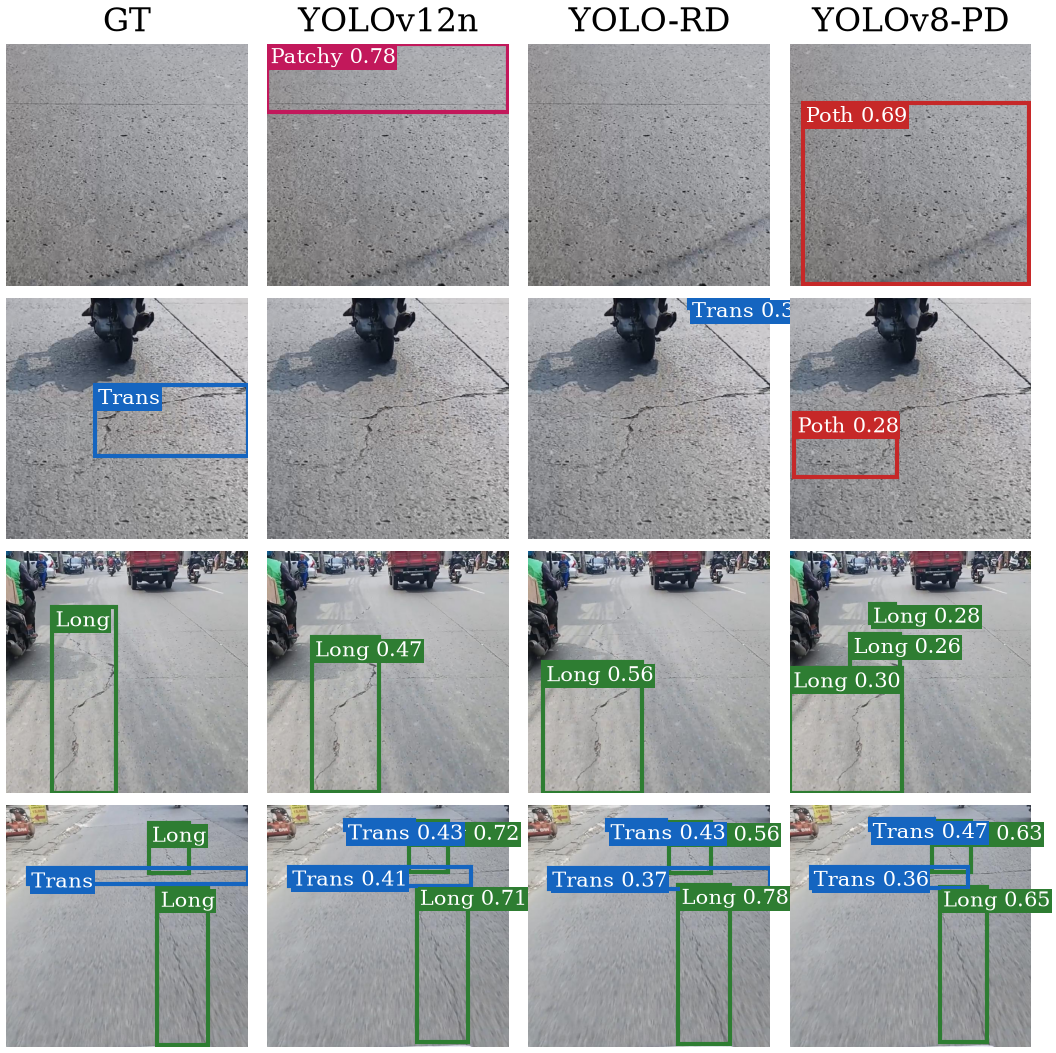
\includegraphics[width=\linewidth]{bab4-contoh-target.png}
\caption{Anotasi acuan dan prediksi pada empat citra target terpilih. Urutan kolom: GT, YOLOv12n, YOLO-RD, dan YOLOv8-PD; ambang tampilan 0,25.}
\label{fig:b4-target}
\end{figure}
Gambar~\ref{fig:b4-target} menampilkan dua contoh dengan kesalahan yang menonjol serta dua contoh dengan retak yang terdeteksi. Singkatan Long, Trans, Poth, dan Patchy pada kotak masing-masing menunjukkan retak memanjang, retak melintang, lubang, dan jalan bertambal. Prediksi tetap menampilkan kategori keluaran model enam kelas, sehingga label jalan bertambal dapat muncul meskipun tidak masuk metrik utama empat kelas.

Pada baris pertama, citra tidak memiliki anotasi kerusakan. YOLOv12n menghasilkan prediksi jalan bertambal dan YOLOv8-PD menghasilkan prediksi lubang, sedangkan YOLO-RD tidak menampilkan kotak pada ambang yang digunakan. Pada baris kedua, YOLOv12n melewatkan retak melintang beranotasi. YOLO-RD menghasilkan kotak retak melintang kecil dengan lokasi yang tidak sesuai, sedangkan YOLOv8-PD memprediksi lubang.

Pada baris ketiga, ketiga model mendeteksi retak memanjang, tetapi YOLOv8-PD menampilkan lebih dari satu kotak. Baris keempat memuat dua anotasi retak memanjang dan satu anotasi retak melintang. Prediksi menangkap retak tersebut, tetapi juga menampilkan kotak retak melintang tambahan. Contoh ini membantu membedakan objek terlewat, kekeliruan kategori, dan kotak tambahan; jumlah baris tidak mewakili frekuensi kesalahan pada seluruh target.

Perbedaan tampilan perkerasan, sudut pengambilan gambar, dan pencahayaan dapat menjadi konteks perubahan domain sebagaimana dibahas pada Bab~\ref{bab:tinjauan-pustaka}. Namun, eksperimen ini tidak mengubah faktor tersebut satu per satu. Penurunan mAP konsisten dengan adanya kesenjangan kinerja antardataset, tetapi tidak menentukan besarnya kontribusi tekstur, pencahayaan, atau lokasi. Kinerja transfer juga tidak dapat diatribusikan langsung kepada modul perhatian tanpa eksperimen yang mengisolasi modul itu.

\subsection{Keterkaitan hasil dan keterbatasan penelitian}
Rumusan masalah pertama dijawab melalui hasil agregat dan per kelas pada sumber, disertai perbandingan konfigurasi label. YOLO-RD menghasilkan mAP enam kelas tertinggi pada pengujian ini. Penambahan label pengecoh tidak menunjukkan manfaat yang konsisten terhadap empat kelas kerusakan ataupun jumlah tumpang tindih yang diperiksa. Kedua temuan tersebut perlu dipisahkan karena mengukur aspek yang berbeda.

Rumusan masalah kedua dijawab oleh perbandingan parameter, GFLOPs, dan estimasi FPS. YOLO26n paling kecil menurut parameter dan GFLOPs, sedangkan YOLOv8-PD memiliki estimasi FPS tertinggi. Rumusan masalah ketiga dijawab oleh penurunan kinerja seluruh model dan perubahan peringkat pada target. YOLOv12n memberikan hasil transfer tertinggi pada empat kelas kerusakan yang sama.

Kekuatan kesimpulan dibatasi oleh satu \textit{seed}, perbedaan kapasitas, transfer bobot pralatih, AMP, dan implementasi rekonstruksi. Pengaturan otomatis optimizer juga tidak menjamin seluruh model memiliki konfigurasi efektif identik. Oleh sebab itu, perbedaan skor tidak dinyatakan signifikan secara statistik dan tidak diperlakukan sebagai pengaruh murni satu komponen arsitektur.

Data target mencakup lokasi terbatas di Kabupaten Bandung dan dianotasi oleh satu orang tanpa pengukuran kesepakatan antar-anotator. Citra berasal dari video, sedangkan tingkat kemiripan antarbingkai belum diukur dalam analisis ini. Hasil pada 307 citra tersebut tidak digeneralisasi sebagai kinerja seluruh jalan Indonesia. Evaluasi yang lebih luas diperlukan untuk menilai kestabilan peringkat pada lokasi dan kondisi perekaman lain.

F1 yang dilaporkan mengikuti titik operasi hasil optimasi kurva pada bagian data yang dievaluasi. Nilainya tidak mewakili ambang penerapan yang telah ditetapkan dari validasi sumber. Estimasi FPS juga berasal dari validator pada GPU desktop, bukan pengujian aplikasi jalan secara langsung. Batas-batas ini menjadi dasar penarikan kesimpulan dan saran pengembangan pada bab berikutnya.
